\section{Cahier des Charges}

Le projet se concentre sur une partie restreinte du récepteur LIN, uniquement pour la réception de trames de type \textbf{« écriture »}, avec une \textbf{entrée LIN unique} et une vitesse fixée à \SI{19200}{bit/s}. La distinction maître/esclave et la connexion physique complète ne sont pas traitées.

\subsubsection*{Limitations et simplifications :}
\begin{itemize}
    \item Pas de gestion de perte d'octets,
    \item Vérification des bits start/stop par un seul échantillon,
    \item Pas de contrôle de parité ni de vérification du checksum.
\end{itemize}

\subsubsection*{Fonctionnalités attendues :}
\begin{itemize}
    \item Conversion série → parallèle (données de 8 bits) pour un microprocesseur,
    \item Possibilité de \textbf{filtrer les messages} grâce à un registre de comparaison \texttt{SelAdr} (8 bits),
    \item Signalisation de fin de réception (\texttt{M\_Received}) uniquement si l'identifiant reçu correspond à \texttt{SelAdr},
    \item Réinitialisation des compteurs et effacement des messages non valides.
\end{itemize}

\subsubsection*{Gestion des messages :}
\begin{itemize}
    \item Un seul message peut être stocké à la fois (FIFO),
    \item Les octets doivent être accessibles dans leur ordre d'arrivée, même si le message est encore en cours de réception,
    \item Tous les octets doivent être mémorisés, indépendamment du filtrage,
    \item Le récepteur doit déterminer la fin du message et l'indiquer au microprocesseur.
\end{itemize}

\subsubsection*{État du récepteur :}  
Accessible par registre ( ETAT ) à tout moment, il doit indiquer :
\begin{itemize}
    \item si un message a été reçu (après filtrage),
    \item le nombre d'octets reçus,
    \item les erreurs simples de réception (bits START/STOP, durée du \textit{synchro break}).
\end{itemize}

Après lecture du registre d'état, les champs sont réinitialisés (sauf le compteur d'octets reçus).

\subsubsection*{Contraintes supplémentaires :}
\begin{itemize}
    \item Interface physique avec le microprocesseur imposée,
    \item Caractéristiques fonctionnelles, physiques et temporelles définies,
    \item Temps d'échanges précisés pour assurer la compatibilité avec l'environnement.
\end{itemize}

\begin{figure}[H]
    \centering
    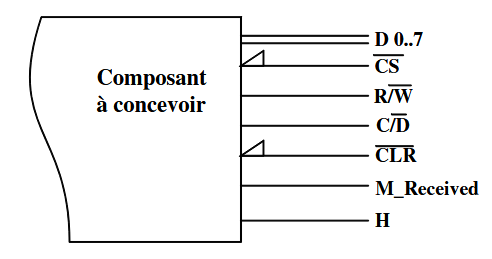
\includegraphics[width=0.8\linewidth]{images/CDC/Compo_concevoir.png}
    \caption{Interface microprocesseur associée au circuit à concevoir}
    \label{fig:placeholder}
\end{figure}

\begin{figure}[H]
    \centering
    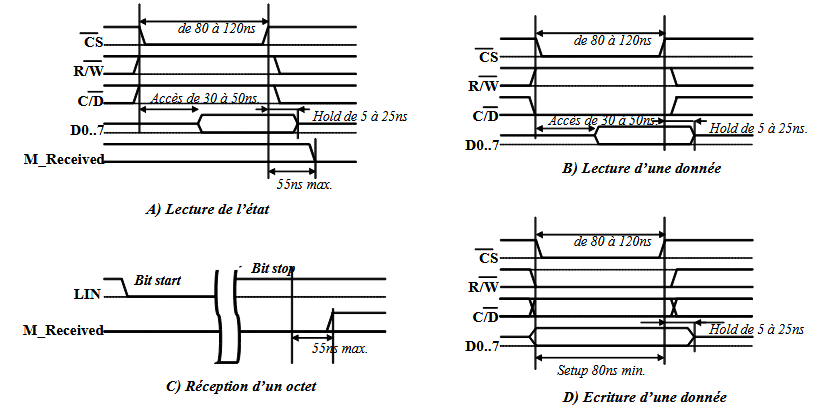
\includegraphics[width=0.8\linewidth]{images/CDC/Chrono.png}
    \caption{Chronogrammes des échanges entre le circuit et son environnement}
    \label{fig:placeholder}
\end{figure}

% Page 2 TD DAVY
\begin{figure}[H]
    \centering
    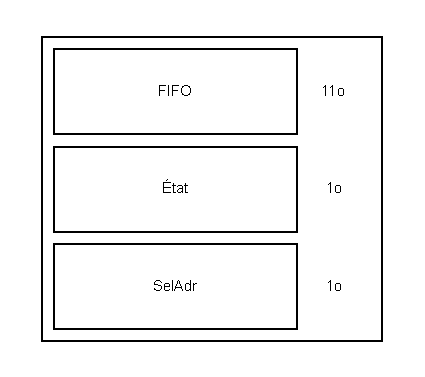
\includegraphics[width=0.8\linewidth]{images/CDC/Schema_Fifi_etat.pdf}
    \caption{Schema Conception Registre interne Système}
    \label{fig:placeholder}
\end{figure}

